% !TEX program = xelatex
\documentclass[a4paper,UTF8]{ctexart}
\usepackage[version=4]{mhchem}
\usepackage[UTF8]{ctex}
\usepackage{fontspec}
\usepackage{geometry}
\usepackage{graphicx}
\setmainfont{SimSun}
\setlength{\parindent}{0em}
\geometry{textwidth=15cm}
\geometry{hcentering}
\begin{document}
\begin{center}
{\huge 我的化学笔记}
\end{center}

\section{氢和稀有气体}
稀有元素:自然界中含量少和分布稀少,被人们发现较晚,难以从矿物中提取或是在工业上制备和应用较晚的元素
\subsection{稀有元素分类}
稀有元素:

(1)轻稀有元素:Li,Rb,Cs,Be

(2)分散性稀有元素:Ga,In,Tl,Se,Te

(3)高熔点稀有元素:Ti,Zr,Hf,V,Nb,Ta,Mo,W

(4)稀土元素:Sc,Y,La及镧系元素

\subsection{化合态和游离态}
游离态:

(1)气态非金属单质

(2)固态非金属单质

(3)金属单质

注:

过冷状态:液态物质在温度降低到凝固点而仍不发生凝固或结晶等相变的现象。(Cs,Ga)


\subsection{单质的制取方法}
1.物理分离法

淘洗黄金,分离氧气氮气

2.热分解法

热稳定性差的某些金属化合物直接加热

$$ \ce{2Ag2O ->[\Delta] 4Ag(s) + O2}$$
$$ \ce{HgS(s) + O2 ->[\Delta]  Hg(l) + SO2(g)}$$

热分解法还用于制备某些高纯单质

$$ \ce{Zr(\text{粗}) + 2I2 ->[600^\circ C] ZrI4 ->[1800^\circ C] Zr(\text{纯}) + 2I2} $$
3.还原法

使用还原剂制取单质的方法叫做还原法。

$$ \ce{MgO(s) + C ->[\Delta] Mg + CO\ce{^}}$$
$$ \ce{Fe2O3 + 2Al ->[\Delta] 2Fe + Al2O3} $$

4.电解法

活泼金属和非金属单质的制备可采用电解法。

$$ \ce{2Al2O3(\text{熔体}) ->[\text{电解}][Na3AlF4,960^\circ C] 3S + 2H2O} $$ 

5.氧化法

用氧化剂制取单质的方法。如制取S:

$$ \ce{3FeS2 + 6C + 8O2 ->[\Delta] Fe3O4 + 6CO2\ce{^} + 6S\ce{^}} $$

也可从\ce{H2S}制取S:

$$ \ce{2H2S + 3O2 -> 2SO2 + 2H2O} $$
$$ \ce{ 2H2S + SO2 ->[CaT][300^\circ C] 3S + 2H2O} $$

\subsection{氢}
\subsubsection{氢原子的成键效应}

1.失去价电子

\ce{H+}半径小,具有很强电场,极化作用很强。

2.结合一个电子

这是\ce{H}与活泼金属形成离子型氢化物如\ce{NaH}、\ce{CaH2}的成键特征

3.形成共价化合物

与其他非金属形成共价型氢化物(\ce{HCl}、\ce{H2S}、\ce{NH3})。

\subsubsection{氢的性质和用途}

性质:

1.溶解度:氢在水中溶解度很小,在金属中溶解度却很大。

2.活泼性:在常温下不活泼。原因是氢原子半径小,无内层电子,所以共用电子对直接受核作用,形成的$\sigma$键很牢固,\ce{H2}的解离能很大。

3.与金属:加热时,与碱金属、碱土金属化合形成离子型氢化物(性质见碱金属/碱土金属部分);\\在过渡型氢化物中,氢以三种形式存在:\\·原子状态存在于金属晶格中\\·氢的价电子进入氢化物导带,以\ce{H+}形式存在\\·氢从氢化物导带中得一个电子,以\ce{H-}形式存在\\高温下,\ce{H2}作为还原剂与氧化物或氯化物反应,还原某些金属和非金属。


用途:

氢的扩散性好,导热性强;熔沸点均低,难液化,可作超低温制冷剂;热值高可作高能燃料。

与碱金属、碱土金属化合形成离子型氢化物(性质见碱金属/碱土金属部分)

化工上,氢气和用于生产甲醇。
$$ \ce{CO(g) + 2H2(g) ->[\text{催化加压}][\text{加热}] CH3OH} $$

食品工业上,则可用于有机物催化加氢。


$$ \ce{WO3 + 3H2 ->[\text{高温}] W + 3H2O} $$
$$ \ce{SiHCl3 + H2 ->[\text{高温}] Si + 3HCl} $$

4.与非金属:绝大多数p区元素与\ce{H2}反应生成共价型氢化物,它们在固态多数属于分子晶体,故又称分子型氢化物;它们大多是无色的,熔沸点较低;它们的物理性质相似,但化学性质显著不同。

5.检验:氢气能让粉红色\ce{PdCl2}水溶液迅速变黑(析出金属钯粉)

$$ \ce{PdCl2(aq) + H2(g) ->[\text{高温}] Pd(s)\ce{v} + 2HCl(aq)} $$

6.温度影响:高温下,氢分子分解为原子氢,具有极强还原性。

\subsubsection{氢气的制备}

实验室里,用\ce{Zn}与盐酸、稀硫酸作用制取氢气;

军事上使用\ce{CaH2}与水反应制取氢气。

工业上,主要有:

1.矿物燃料转化法:

制备水煤气:

$$ \ce{CH4(g) + H2O(g) ->[CaT][700-800^\circ C] CO(g) + 3H2} $$
$$ \ce{C(s) + H2O(g) ->[1000^\circ C] CO(g) + H2(g)} $$

将水煤气与水蒸气反应

$$ \ce{CO(g) + H2O(g) ->[400-600^\circ C][\ce{Fe},\ce{Cr}\text{催化剂}] CO2(g) + H2(g)} $$

本质上,每一步都是在让\ce{C}夺走水中的\ce{H}

该法制氢伴随大量\ce{CO2}产生。

2.电解法

电解\ce{NaOH}溶液,则在阴极产生氢气,阳极产生氧气。

\subsection{稀有气体}

稀有气体:0族元素所对应的气体单质。

\subsubsection{稀有气体的性质和用途}

稀有气体原子间存在微弱的色散力,作用力随着原子序数增大而增大(因为分子变形性增大)。所以,稀有气体的物理性质(熔沸点、临界温度、溶解度)也随着原子序数增大而增大。

1.氦(\ce{He})

用来代替氧气瓶中\ce{N2},防止潜水员“潜水病”。

2.氖(\ce{Ne})和氩(\ce{Ar})

霓虹灯、保护气、冷冻剂。

3.氪(\ce{Kr})和氙(\ce{Xe})

特种光源、麻醉剂。

4.氡(\ce{Rn})

有放射性,可用于放疗。

\subsubsection{稀有气体化合物}
第一个稀有气体化合物:

$$ \ce{Xe(g) + PtF6(g) -> Xe+[PtF6]-(s)} $$

现在,有稀有气体卤化物、氧化物、含氧酸盐等,大多都与氟化物的反应有关。

稀有气体氟化物:

$$ \ce{Xe(g) + F2(g) -> XeF_{x}(g)} $$

根据\ce{F}的用量和时间长短,可分别制得$x=2,4,6$的化合物;反应中若进入湿气,则生成爆炸的\ce{XeO3}。

\ce{XeF2}与水反应生成\ce{Xe}和\ce{HF}、\ce{O2};\ce{XeF4}、\ce{XeF6}则与水反应生成固态的\ce{XeO3}

\ce{Xe}的氟化物是优良的氟化剂,如:

$$ \ce{Pt + XeF4 -> PtF4 + Xe} $$

\ce{Xe}的三种氟化物均为强氧化剂,如:

$$ \ce{XeF2 + H2O2 -> Xe + 2HF + O2\ce{^}} $$

$$ \ce{6HCl + XeF6 -> 3Cl2\ce{^} + 6HF + Xe} $$

$$ \ce{6HCl + XeF6 -> 3Cl2\ce{^} + 6HF + Xe} $$

需要注意的是\ce{Xe}的氟化物的分子结构。\ce{XeF4}中有中心原子的8个电子,每个\ce{F}原子提供一个价电子,价层有$\frac{8+(4\times1)}{2}=6$对电子,为八面体结构。两对孤电子占据对角,四个成键电子对占据四个顶点,为正方形,\ce{Xe}位于正方形中心。



\section{碱金属和碱土金属元素}

\subsection{碱金属和碱土金属通性}

$IA$和$IIA$族元素均只有1到2个s电子,同一周期中,半径大、电荷少。所以,它们的金属晶体中金属键不牢固,单质熔沸点低,硬度小。由于碱土金属比碱金属原子半径小、原子电荷多,因此碱土金属的熔沸点都比碱金属高,密度、硬度都比碱金属大。

总的来说,从上到下熔沸点降低、密度增加、硬度减小、电负性降低、$E^{\theta}(\ce{M2+}/\ce{M})$绝对值增加,还原性增加。

然而,\ce{Li/Li+}的标准电极电势反常,因为其原子半径小,很容易与\ce{H2O}结合放出能量,水合焓代数值最小,



\section{过渡元素(二)}

\subsection{铜族元素}

\subsubsection{铜族元素通性}

铜族元素位于元素周期表ds区IB族,包含铜(\ce{Cu})、银(\ce{Ag})、金(\ce{Au})、錀(\ce{Rg})。

铜、银主要以硫化物、氧化物矿的形式存在;铜、银、金均有单质状态存在的矿物。

铜族元素原子价层电子构型为$(n-1)d^{10}ns^{1}$,氧化数有+1,+2,+3;

铜、银、金最常见的氧化数分别为+2、+1、+3 。(铜、金非+1的原因可参考它们的氧化电极电势,并且\ce{Cu^{+}}在水中容易与水结合,导致能量变化,易歧化为0、+2价)

$$ E^{\Theta}_{A}/V \quad \ce{Cu^{3+} \overset{2.4}{\text{------}} Cu^{2+} \overset{0.159}{\underset{}{\text{------}}} Cu+ \overset{0.520}{\underset{}{\text{------}}} Cu}$$

$$ E^{\Theta}_{A}/V  \quad \ce{Ag^{3+} \overset{1.8}{\underset{}{\text{------}}} Ag^{2+} \overset{1.980}{\underset{}{\text{------}}} Ag+ \overset{0.7991}{\underset{}{\text{------}}} Ag} $$




铜族金属离子有较强的极化力,本身变形性大,二元化合物有相当的共价型(如\ce{CuCl2}为共价化合物)。

与其他过渡金属类似,易形成配合物。\\$\Delta$原因:(1)过渡元素有能量相近的未充满的(n-1)d,ns,np价轨道,属于同一能级组,可以通过不同杂化方式形成杂化轨道,接受配体提供的孤对电子,有的还可以形成d-p反馈$\pi$键。(2)过渡金属电子层数增加慢,钻穿效应强,有效核电荷数多,有利于作为中心原子吸引配体。

\subsubsection{铜族元素单质}
熔沸点相对较低,硬度小,有极好延展性和可塑性;导热、导电能力极强,\ce{Cu}是最通用导体。

银、金熔体能从空气中吸收大量氧气,冷凝时又释放。

银、铜、金能与多种金属形成合金。

银、铜、金的化学活泼性差;\ce{Cu}在潮湿空气中生成铜绿:

$$ \ce{2Cu + O2 + CO2 -> Cu2(OH)2CO3} $$

银的化学活泼性在铜、金之间,在室温下不与氧气、水反应,在高温不与氢、氮、碳反应,与卤素反应较慢。在室温下与含有\ce{H2S}的空气反应会生成深色\ce{Ag2S}。

$$ \ce{4Ag + 2H2S + O2 -> 2Ag2S + 2H2O} $$

铜,银仅与氧化性酸反应:与稀硝酸生成硝酸盐和\ce{NO},与浓硝酸生成硝酸盐和\ce{NO2},与热的浓硫酸反应生成\ce{SO2}

高温下与氧气不反应的只有金。

金不溶于单一无机酸,但溶于王水:

$$ \ce{Au + HNO3 + 4HCl ->H[AuCl4] + NO\ce{^} + 2H2O} $$

银遇王水产生\ce{AgCl}薄膜阻止反应继续进行。

\subsubsection{铜的重要化合物}
1.氧化物和氢氧化物\\

\ce{CuO}:

加热分解硝酸铜和碳酸铜可得黑色\ce{CuO};\ce{Cu(OH)2}受热分解脱水也生成\ce{CuO}

\ce{CuO}加热可分解为暗红色\ce{Cu2O}

$$ \ce{4CuO ->[1000^\circ C] 2Cu2O + O2} $$

\ce{CuO}是高温超导材料。\\

\ce{Cu(OH)2}:

\ce{Cu(OH)2}显两性(以弱碱性为主),既溶于酸也溶于浓强碱,在强碱中生成四羟基合铜离子。

\ce{[Cu(OH)4]2-}可被葡萄糖还原为暗红色的\ce{Cu2O}

$$ \ce{[2Cu(OH)4]2- C6H12O6 -> Cu2O\ce{v} + C6H12O7 + 4OH- + 2H2O} $$

\ce{Cu(OH)2}易溶于氨水,生成深蓝色\ce{[Cu(NH3)4]^{2+}}。\\

\ce{CuCl}和\ce{Cu2O}:

\ce{CuCl}难溶于水,溶于氨水和浓盐酸并生成配合物。

向\ce{CuCl}的盐酸冷溶液中加入\ce{NaOH},生成黄色\ce{CuOH}沉淀,但沉淀很快变为橙色,最后变为红色\ce{Cu2O}。

\ce{Cu2O}热稳定性很强,难溶于水,但是易溶于稀酸,并立即歧化为\ce{Cu^{2+}}和\ce{Cu}。

$$ \ce{Cu2O + 2H+ -> Cu^{2+} + Cu + H2O} $$

与盐酸则反应生成难溶于水的\ce{CuCl}

$$ \ce{Cu2O + 2HCl -> CuCl + H2O} $$

溶于氨水,形成无色配离子\ce{[Cu(NH3)2]^{+}}

$$ \ce{Cu2O + 4NH3 + H2O -> [Cu(NH3)2]^{+} + 2OH-} $$

但\ce{[Cu(NH3)2]^{+}}遇到空气就被氧化为深蓝色\ce{[Cu(NH3)4]^{2+}}

$$ \ce{4[Cu(NH3)2]^{+} + O2 + 8NH3 + 2H2O -> 4[Cu(NH3)4]^{2+} + 4OH-} $$\\

\ce{[Cu(NH3)2]OAc}可以吸收\ce{CO}。

$$ \ce{[Cu(NH3)2]OAc + CO + NH3 <=>[\text{低温加压}][\text{升温减压}] [Cu(CO)(NH3)3]OAc} $$

\ce{Cu2O}可用作红色颜料。\\

2.盐类

(1)氯化亚铜

向热的浓盐酸中用铜还原\ce{CuCl2}可以生成无色\ce{[CuCl2]-}配合物,用水稀释即可生成白色\ce{CuCl}沉淀。

$$ \ce{Cu + Cu^{2+} + 4Cl- -> 2[CuCl2]-} $$

$$ \ce{2[CuCl2]- -> 2CuCl + 2Cl-} $$

用还原剂\ce{SnCl2}也可以得到\ce{CuCl}。

$$ \ce{2CuCl2 + SnCl2 -> 2CuCl\ce{v} + SnCl4} $$

另外,\ce{CuCl}还可以吸收\ce{CO}生成氯化羰基亚铜(\ce{[Cu(CO)Cl]\cdot H2O})

$$ \ce{CuCl + CO + H2O -> [Cu(CO)Cl]\cdot H2O} $$

该反应可用于测定有机反应中\ce{CO}的产生量。

(2)氯化铜

\ce{CuCl2}是一种棕黄色固体,可由单质直接化合而成,是一种共价化合物,结构为\ce{CuCl4}组成的长链。

\begin{figure}[ht]
	\centering
	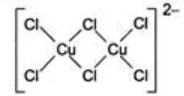
\includegraphics[width=0.3\textwidth]{figure//Cu结构.png}
	\caption{Cu结构.png}
	\label{fig:Cu结构}
\end{figure}

\ce{CuCl2}不仅易溶于水,而且易溶于有机溶剂,如乙醇,丙酮等。在很高浓度\ce{CuCl2}溶液中,可形成黄色配合物\ce{[CuCl4]^{2-}},显黄色。

$$ \ce{Cu^{2+} + 4Cl- -> [CuCl4]^{2-}} $$

在\ce{CuCl2}稀溶液中,由于被\ce{[Cu(H2O)4]^{2+}}取代,显浅蓝色。

$$ \ce{[CuCl4]^{2-} + 4H2O -> [Cu(H2O)4]^{2+} + 4Cl-} $$

所以,\ce{CuCl2}高浓度溶液常显黄色或黄绿色,这是两种配离子都存在的缘故。

(3)硫酸铜

无水硫酸铜为白色粉末,在水中结晶时为五水合硫酸铜,呈蓝色。五水合硫酸铜(\ce{[Cu(H2O)5]SO4})俗称胆巩,其结构为\ce{[Cu(H2O)4]SO4\cdot H2O},4个水分子与\ce{Cu^{2+}}配位,1个水分子通过氢键与\ce{SO4^{2-}}结合。温度升高,水逐渐脱去。

无水硫酸铜易溶于水,吸水性强,吸水则显出特征性蓝色,可用于测量气体微量水分和作为干燥剂。\ce{CuSO4}由于铜离子水解而呈弱酸性。

\ce{CuSO4}具有杀菌性,可制备波尔多液。\\

3.配合物

(1)\ce{Cu}(I)的配合物:

\ce{Cu}(I)通常形成配位数为2的配合物,常见的有:

\ce{[Cu(SCN)2]+},\ce{[CuCl2]-},\ce{[Cu(NH3)2]+},\ce{[Cu(S2O3)]^{2-}},\ce{[Cu(CN)2]-}

由于\ce{Cu+}的价电子结构为$d^{10}$型,形成的配离子基本无色,大多配合物溶液有吸收\ce{CO}、烯烃、炔烃和释放的能力。

$$ \ce{[Cu(NH2CH2CH2OH)2]+ + C2H4 <=> [Cu(NH2CH2CH2OH)2(C2H4)]+} \Delta _{f}H^{\Theta}_{m}<0$$

该反应常用于石油中分离烯烃。

(2)\ce{Cu}(II)的配合物:

\ce{Cu}(II)与单齿配体通常形成配位数为4的正方形配合物,例如\ce{[CuCl4]2-},\ce{[Cu(NH3)4]^{2+}},\ce{[Cu(H2O)4]^{2+}}。

过量氨水与\ce{Cu^{2+}}盐溶液反应可以生成\ce{[Cu(NH3)4]^{2+}}。

$$ \ce{[Cu(H2O)4]^{2+} + 4NH3 -> [Cu(NH3)4]^{2+} + 4H2O} $$





\end{document}
